\section{Zielsetzung}
\label{sec:Zielsetzung}

In diesem Versuch werden für diese beiden Strahlungsarten, die $\gamma$- und $\beta$-Strahlung, auf ihre Wechselwirkungsmechanismen mit Materie näher eingegangen. Als erstes soll das exponentielle Absorptionsgesetz bestätigt werden. Danach sollen die Absorptionskoeffiziente für verschiedene Materialien bestimmt werden. Am Ende wird die Maximalenergie eines $\beta$-Teilchens bestimmt.

\section{Theorie}
\label{sec:Theorie}

Wechselwirkt energiereiche Strahlung mit Materie, so kommt es zu Absorptionserscheinungen. Eine wichtige Größe ist dabei der Wirkungsquerschnitt $\sigma$, welcher wie eine fiktive Fläche bei dem Auftreffen eines Teilchens auf diese zu Wechselwirkung führt.
Wird angenommen, dass die Elektronen die Wechselwirkungszentren im Absorbermaterial darstellen, lässt sich der Wirkungsquerschnitt nähern:
\begin{align}
\sigma &= \frac{\mu}{n} = \frac{\mu M}{z N_\text{L} \rho} \\
\tiny \text{$z$: Ordnungszahl, $N_\text{L}$: Loschmidtsche Zahl, }&\text{\tiny $\rho$: Dichte, $M$: Molekulargewicht, $n$: Materieteilchen pro Volumenelement} \nonumber
\end{align}
$\mu$ beschreibt hier den Absorptionskoeffizienten, welcher mit $\sigma$ und $n$ zusammenhängt:
\begin{equation*}
\mu =n \sigma.
\end{equation*}
Das Absorptionsgesetz lautet:
\begin{equation}
\label{eq:eq1}
N(D) =N_0 e^{-\mu D} 
\end{equation}
und ist gültig bei nur einer Wechselwirkung eines einfallenden Teilchens mit dem Absorber oder wenn die mittlere Entfernung zwischen zwei Reaktionen groß gegenüber der Absorberschichtdicke $D$ groß ist. $N_0$ beschreibt die Anzahl der Teilchen, welche pro Zeiteinheit auf die Querschnittsfläche des Absorbers treffen. 

\subsection{\texorpdfstring{$\gamma$}{gamma}-Strahlung und ihre Wechselwirkung mit der Materie}

Die $\gamma$-Strahlung, also Photonenstrahlung, entsteht erst, wenn der Atomkern in einem angeregten Zustand, die noch vorhandene überschüssige Energie, in Form eines oder mehrerer Gammaquanten abgibt. Weil diese Energieniveaus diskrete Zustände besitzen, handelt es sich um ein Linienspektrum. Die Gammaquanten breiten sie sich nur mit der Lichtgeschwindigkeit aus. Es lassen sich viele typische Eigenschaften der elektromagnetischen Strahlung ableiten, wie z.B. Interferenz.

Es treten unterschiedliche Effekte der Gammastrahlung bei der Wechselwirkung mit der Materie. Es gibt Wechselwirkung in Form von Annihilation, elastischer- und inelastischer Streeung, wobei meist nur eine Wechselwirkung zustande kommt. 

\begin{figure}[h!]
	\centering
	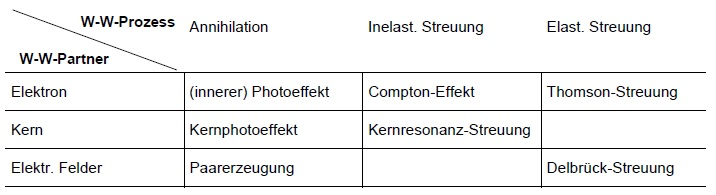
\includegraphics[width=0.9\linewidth]{../../WechselwirkungMaterieGamma}
	\caption{Die Wechselwirkungen der $\gamma$-Quanten, \cite[4]{anleitung704}.}
	\label{fig:wechselwirkungmateriegamma}
\end{figure}

Die wichtigsten Effekte sind im Wesentlichen Compton- und Photo-Effekt und Paarbildung. Sie treten bei unterschiedlichen Wechselwirkungen auf und sind in der Abbildung \ref{fig:wechselwirkungmateriegamma} zu finden. 

Beim Photo-Effekt wird ein inneres Hüllenelektron unter Annihilation des Photons seiner Bindung gelöst. Dieser Effekt tritt auf, wenn die Energie des Photons größer als die Bindungsenergie des Elektrons ist.

Das Photon wird allerdings beim Compton-Effekt nicht vernichtet. Dieser bezeichnet eine inelastische Streeung an einem freien Elektron, welche für eine Richtungs- und Energieänderung sorgt. Das Photon gibt beim Stoß mit einem Elektron nur einen Teil seiner Energie ab. Der Wirkungsquerschnitt $\sigma_\text{com}$ berechnet sich für diese Art von Wechselwirkung wie folgt:
\begin{equation*}
\sigma_\text{com} = 2 \pi r_e^2 \left(\frac{1+\epsilon}{\epsilon^{2}}\left[\frac{2(1+\epsilon)}{1+2\epsilon}-\frac{1}{\epsilon}\text{ln}(1+2\epsilon)\right]+\frac{1}{2\epsilon}\text{ln}(1+2\epsilon)-\frac{1+3\epsilon}{(1+2\epsilon)^2}\right)
\end{equation*}
mit \begin{align*}
\epsilon &= \frac{E_\gamma}{m_e0 c^2} \\
r_e &= \frac{e^2}{4 \pi \epsilon_0 m_0 c^2}
\end{align*}
wobei $\epsilon$ das Verhältnis der Quantenenergie $E_\gamma$ zur Ruheenergie des Elektrons ist und $r_e$ der klassische Elektronenradius beschreibt. Außerdem sind $e$ die Elementarladung, $m_0$ die Ruhemasse des Elektrons und $\epsilon_0$ die Influenzkonstante. Durch den Comptoneffekt ergibt sich den Compton-Absorptionskoeffizient $\mu_\text{com}$ zu:
\begin{equation*}
\mu_\text{com} = n\sigma_\text{com}(\epsilon) = \frac{zN_\text{L}\rho}{M}\sigma_\text{com}(\epsilon).
\end{equation*}

Die Paarbildung tritt auf, wenn folgendes gilt:
\begin{equation*}
E_\gamma > 2m_0c^2
\end{equation*}
also wenn die Energie des $\gamma$-Quants doppelt so hoch ist wie die Ruhemasse eines Elektrons $m_0$. Bei Bildung eines Elektrons und eines Positrons wird das Photon annihiliert. 

\begin{figure}[h!]
	\centering
	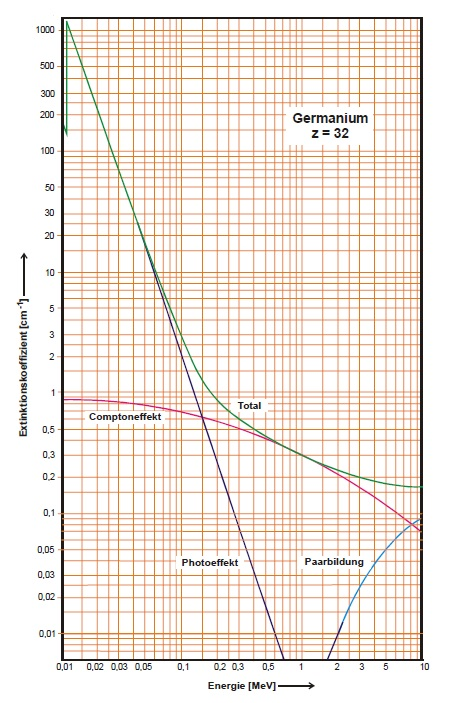
\includegraphics[width=0.7\linewidth]{../../EnergieWechselwirkung}
	\caption{Wechselwirkungen in Abhängigkeit der Energie und des Absorptionskoeffizienten(Germanium), \cite[7]{anleitung704}.}
	\label{fig:energiewechselwirkung}
\end{figure}

In der Abbildung \ref{fig:energiewechselwirkung} ist eine Wechselwirkungeffektüberlagerung dargestellt, wobei für unterschiedliche Energiebereiche unterschiedliche Effekte dominierend sind. 

\subsection{\texorpdfstring{$\beta$}{beta}-Strahlung und ihre Wechselwirkung mit der Materie}

$\beta$-Strahlung ist eine Teilchenstrahlung bestehend aus Elektronen bei der häufigeren $\beta^{-}$-Strahlung oder Positronen bei der $\beta^{+}$-Strahlung. Im Prinzip sind Elektronen, die eine hohe kinetische Energie besitzen.
Die Formeln für diesen Zerfall lauten:
\begin{align*}
\text{n} \rightarrow \text{p} + \beta^{-} + \bar{\nu_e}, \\
\text{p} \rightarrow \text{n} + \beta^{+} + \nu_e.
\end{align*}
Dabei wandelt es sich ein Neutron in ein Proton, Antineutrino und Elektron um. Ein Atomkern emittiert bei einer Nukleonenumwandlung ein Elektron oder Positron, samt passendem Neutrino, wobei die freiwerdende Energie gleichmäßig auf diese verteilt werden, sodass es zu einem kontinuierlichen Spektrum kommt. Die Maximalenergie $E_\text{max}$ ist die gesamte bei dem Zerfall frei werdende Energie. 
Wird $\beta^{-}$-Strahlung absorbiert, gibt es viele Wechselwirkungsprozesse, so dass sich kein einfacher Zusammenhang ergibt. 

Eine erste mögliche Art von Streuung ist die elastische Streuung am Atomkern, also die Rutherfordstreuung. Es handelt sich dabei um eine elastische Streuung mit großer Bahnablenkung bei geringer Energieabnahme.

Die zweite Art von Streuung ist die inelastische Streuung am Atomkern, aufgrund des Coulombfeldes des Kerns wird das $\beta^{-}$-Quant gestreut und es entsteht Bremsstrahlung, da die Energie in Form von elektromagnetischer Strahlung abgegeben wird und diese wiederrum abbremst.

Bei der letzten Art handelt es sich um eine inelastische Streuung an Elektronen im Absorbermaterial. Dies führt zur Ionisation- sowie Anregungsprozesse. Wegen dem dabei auftretenden geringen Energieverlust kann ein Teilchen mehrfach ionisieren.

In der Abbildung \ref{fig:absorptionskurve} ist eine Absorptionskurve qualitativ dargestellt. Für geringe $D$ über der maximalen Reichweite $R_\text{max}$ stellt das Absorptionsgesetz nach \ref{eq:eq1} eine passende Näherung dar. Bei Schichtdicken oberhalb der maximalen Reichweite kommt es jedoch zu starken Abweichungen, die Intensität wird unabhängig von $D$, zum Beispiel die Bremsstrahlung wird entscheidend für die Intensität.
\begin{figure}[h!]
	\centering
	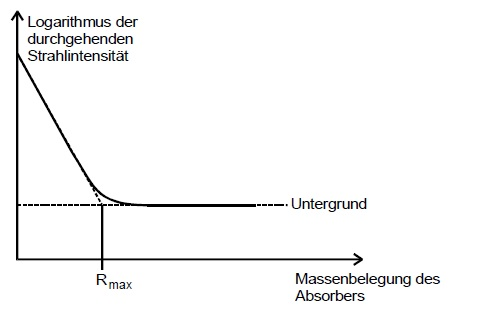
\includegraphics[width=0.7\linewidth]{../../Absorptionskurve}
	\caption{Absorptionskurve eines $\beta^{-}$-Strahlers, \cite[12]{anleitung704}.}
	\label{fig:absorptionskurve}
\end{figure}
Die Massenbelegung des Absorbers aus der Abbildung \ref{fig:absorptionskurve} und die Schichtdicke $D$ errechnen sich durch die Beziehung:
\begin{equation*}
R = \rho D.
\end{equation*}
Weil $R_\text{max}$ durch die Elektronen mit der größten Energie bestimmt wird, kann auch die freiwerdende Gesamtenergie $E_\text{max}$ ermittelt werden. Es lässt sich empirisch ein Zusammenhang zwischen $R_\text{max}$ und $E_\text{max}$ aufstellen:
\begin{equation*}
E_\text{max} = 1,92\sqrt{R_\text{max}^{2}+0,22R_\text{max}}\left[\si{\mega\electronvolt}\right].
\end{equation*}
